\documentclass[a4paper,%
11pt,%
DIV=14,
headsepline,%
headings=normal,
]{scrartcl}

\usepackage[utf8]{inputenc}
\usepackage[T1]{fontenc}
\usepackage[automark]{scrpage2}
\usepackage{graphicx}
\usepackage{lmodern} 
\usepackage{url}
\usepackage{amsmath}
\usepackage{amssymb}
\usepackage{booktabs}
\usepackage{listings}
\usepackage[backend=biber]{biblatex}
\usepackage{tikz}


\lstset{basicstyle=\ttfamily,frame=single}

\newcommand{\exercise}[1]{\section*{Exercise #1}}
\newcommand{\answer}[1]{\subsection*{Answer #1}}

\begin{document}
\usetikzlibrary{shapes,arrows}

\noindent
\hrule height 1px
\vspace*{1ex}
\begin{minipage}[t]{.45\linewidth}
\strut\vspace*{-\baselineskip}\newline

\includegraphics[height=.9cm]{./figs/Inf-Logo_black_en.pdf}
\includegraphics[height=.9cm]{.//figs/par-logo}
\end{minipage}
\hfill
\begin{minipage}[t]{.5\linewidth}
\flushright{
Research Group for Parallel Computing\\%
Faculty of Informatics\\%
TU Wien}
\end{minipage}
\vspace*{1ex}

\hrule 

\vspace*{2ex}

\begin{center}
{\LARGE\textbf{Advanced Multiprocessor Programming}}\\
{\large{}%
  Summer term 2021\\
  Batch 2\\
}
\end{center}

\hrule 
\vspace*{1ex}

\noindent
1: Daniel, Schloms, 11701253\\

\vspace*{1ex}
\hrule 

\exercise{21}

Why is quiescent consistency compositional?\\
\\
Definitions according to the book/slides:\\
Quiescent consistency: Method calls separated by period of quiescence should appear to take effect in their real-time order.\\
Compositional consistency: If two objects are consistent (e.g. quiescently), then any system using these objects together is also consistent.\\
\\
Assume an object $O$ that is made up of two "sub-objects" $O_A$ and $O_B$. For one, calls to $O_A$ and $O_B$ are already quiescently consistent (prerequisite). Furthermore, any calls going to either $O_A$ or $O_B$ must be a call to the overarching object $O$, so if $O$ experiences quiescence, $O_A$ and $O_B$ must as well. If the $O$ was not quiescently consistent, then calls separated by periods of quiescence could return "garbage", however, since when $O$ experiences quiescence, and $O_A$ and $O_B$ must experience quiescence at the same, this would mean that either $O_A$ or $O_B$ is not quiescently consistent, which is a contradiction. If $O$ receives concurrent calls, then $O_A$ and $O_B$ can either both receive calls or only one object receives calls. If only one object receives calls, then quiescent consistence holds because of the quiescent consistence of the receiving sub-object. If both sub-objects receive concurrent calls, then $O$ can return either result first anyway because it does not have to care about the order.
 
\exercise{22}

A memory object holding two quiescently consistent registers is also quiescently consistent (see Ex. 21), does the converse hold (quiescently consistent object implies quiescently consistent subregisters)?\\
\\
No, because there is the possibility that the object only returns values from single register that behaves quiescently consistent. If that register was quiescently consistent and the other register wasn't, the whole object would still behave quiescently consistent, but no assumtions about the ``unused`` register can be made.

\exercise{23}

An example for a quiescently consistent execution that is not sequentially consistent can be seen in figure \ref{fig:qc_not_seq}. We start by writing x in the first thread and then we don't go quiescent. The first thread writes y after x, but reads x in the last call. This is still quiescently consistent, as there was no period of quiescence, so returning x is still legal. It is however not sequentially consistent, as the program order of the first thread was not kept.\\
\\
An example for a sequentially consistent execution that is not quiescently consistent can be seen in figure \ref{fig:seq_not_qc}. Every call is seperated by a quiescent period, yet the upper thread dequeues x instead of y, which would violate the specific condition of quiescent consistency. It is still sequentially consistent, since the order of both enqueue calls are unrelated by program order (different threads) and thus the order of those 2 calls can be changed around.

\begin{figure}[h]
\hspace*{8em}
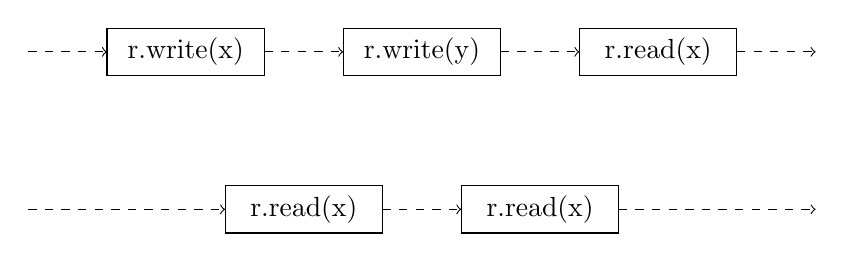
\begin{tikzpicture}

% Thread A
\draw[dashed, ->] (0,0) -- (1,0);
\draw[dashed, ->] (3,0) -- (4,0);
\draw[dashed, ->] (6,0) -- (7,0);
\draw[dashed, ->] (9,0) -- (10,0);
\draw (1,-0.3) rectangle (3,0.3) node[pos=.5] {r.write(x)};
\draw (4,-0.3) rectangle (6,0.3) node[pos=.5] {r.write(y)};
\draw (7,-0.3) rectangle (9,0.3) node[pos=.5] {r.read(x)};

% Thread B
\draw[dashed, ->] (0,-2) -- (2.5, -2);
\draw[dashed, ->] (4.5,-2) -- (5.5,-2);
\draw[dashed, ->] (7.5,-2) -- (10,-2);
\draw (2.5,-2.3) rectangle (4.5,-1.7) node[pos=.5] {r.read(x)};
\draw (5.5,-2.3) rectangle (7.5,-1.7) node[pos=.5] {r.read(x)};


\end{tikzpicture}
\caption{Quiescently consistent, but not sequentially consistent}
\label{fig:qc_not_seq}
\end{figure}

\begin{figure}[h]
\hspace*{8em}
\begin{tikzpicture}

% Thread A
\draw[dashed, ->] (0,0) -- (4,0);
\draw[dashed, ->] (6,0) -- (7,0);
\draw[dashed, ->] (9,0) -- (10,0);
\draw (4,-0.3) rectangle (6,0.3) node[pos=.5] (enqx) {q.enq(x)};
\draw (7,-0.3) rectangle (9,0.3) node[pos=.5] (deqx) {q.deq(x)};

% Thread B
\draw[dashed, ->] (0,-2) -- (1, -2);
\draw[dashed, ->] (3,-2) -- (10,-2);
\draw (1,-2.3) rectangle (3,-1.7) node[pos=.5] (enqy) {q.enq(y)};


\end{tikzpicture}
\caption{Sequentially consistent, but not quiescently consistent}
\label{fig:seq_not_qc}
\end{figure}

\exercise{24} 

\answer{First History}

Quiescently consistent?\\
Yes, because the first 3 calls overlap, so both reads return valid values for quiescent consistency.\\
Sequentially consistent?\\
Yes, because the threads' program orders are still preserved and the 2 writes can be ordered in any order.\\
Linearizable?\\
Yes, each call does appear to take effect instantaneously at some moment between invocation and response. B writes 1 then A reads 1 then C writes 2 then B reads 2.

\answer{Second History}
Quiescently consistent?\\
Yes, same reason as in the first history, the first 3 calls overlap, so either write value is valid for the second read.\\
Sequentially consistent?\\
Yes, again for the same reason as in the first history, both writes are still unrelated by program order and thus can be ordered in any way.\\
Linearizable?\\
Yes, we can still find linearization points for this history. C writes 2 then B writes 1 then A reads 1 then B reads 1.

\exercise{27}
\label{ex27}

The issue arises when some thread $t_1$ tries to enqueue some value \texttt{x}, passes the while check but then falls asleep before assigning \texttt{items[slot] = x}. Now a second thread $t_2$ enqueues \texttt{y} and completes the \texttt{enq()} call completely. If another thread now tried to call \texttt{deq()}, it would cause an \texttt{EmptyException}, as the head still points to an item that has yet to be filled by $t_1$. However, since an enqueue operation was already completed before, this means that the principle of linearizability is violated.

\exercise{32}

\answer{a)}
Show that \texttt{enq()} cannot have a linearization point at line 15.\\
\\
Assume 2 threads $t_1$ and $t_2$ with the following execution order\\
$t_1$ line 15 then $t_2$ line 15 then $t_2$ line 16\\
If another thread $t_3$ then dequeues at that moment and reaches the tail, the value will be that of $t_2$ even if $t_1$ executed line 15 earlier.

\answer{b)}
Show that \texttt{enq()} cannot have a linearization point at line 16.\\
\\
Assume 2 threads $t_1$ and $t_2$ with the following execution order\\
$t_1$ line 15 then $t_2$ line 15 then $t_2$ line 16 then $t_1$ line 16\\
If another thread $t_3$ then dequeues at that moment and reaches the tail, the value will be that of $t_1$ even if $t_2$ executed line 16 earlier.

\answer{c)}
Is \texttt{enq()} linearizable at all?\\
\\
Yes, \texttt{enq()}, is still linearizable, just not at a fixed point. Depending on the execution, it must happen either on line 15 or 16. In contrast to Exercise 27, an enqueue operation that has finished will always be visible to subsequent method calls. This is because even if memory was reserved by a thread that falls asleep before assigning a value, a dequeue operation will just skip that value and dequeue the value of the finished enqueue call.

\exercise{52}

Show that with sufficiently many $n$-thread binary consensus objects and atomic registers one can implement $n$-thread consensus over $n$ values.\\
\\
This can be done by treating the values as binary numbers and deciding the value bit by bit, so 1 binary consensus unit is used per bit. Each thread then publishes its value in a public array and we start deciding. If a thread sees that the bit it was proposing won, its public value stays the same and it moves on to the next bit. If the thread loses, it checks the public array for values that have the same bits up until the point where it lost the decision. This way, each round those values that no longer match are eliminated and replaced with values that are still in the race, until every value in the public array is the same at the latest at the last bit, then this value can then be returned.

\exercise{53}

Show that the \texttt{Stack} class has a consensus number of exactly two.\\
\\
This proof is almost the same as the proof for FIFO queues from the book (5.4).\\
\\
First we prove least two-thread consensus with two possible values, \texttt{WIN} and \texttt{LOSE}. As a consensus class we just use the one from the book for FIFO queues (Figure 5.7) and change queue to stack, and enqueue to push and dequeue to pop respectively. Additionally, we have to push \texttt{LOSE} before \texttt{WIN} in the initializing method since a stack is LIFO.
\begin{itemize}
\item Consistency: there are 2 ways in which the returned values could differ
	\begin{itemize}
	\item Both threads pop \texttt{WIN}, contradicts stack operation itself
	\item Both threads pop \texttt{LOSE}, contradicts stack operation itself
	\end{itemize}
\item Validity: the thread that pops \texttt{WIN} must have stored the winning value in the \texttt{proposed[]} array before another thread can pop any value.
\item Wait-free: No loops in the protocol
\end{itemize}

Then we prove that the consensus number is exactly 2.\\
\\
Here the proof is again almost the same as in the book (Theorem 5.4.1), so the same basic assumtions are made (e.g. A moves first should lead to 0-valent state etc.). We have to show that there is no critical section when using 3 threads. First we assume that we are in a critical section and show that there is no way to get into an univalent state with a third thread C.\\
First we look at the case that both threads A and B. In that case, C can't see which thread popped first.\\
Then we assume A pushes and B pops. If A moves first, B will pop that value of the stack and C will not be able to tell anything from an empty stack. If B moves first, then 0 will be on the stack, but C can't tell if B popped first or if B has yet to move.\\
Lastly, if A and B both push, we can just let A and B run until A and B pop both values of the stack again, then C will again find an empty stack from which it can tell nothing about the order of the moves of A and B.

\exercise{54}

Show that the FIFO queue class with \texttt{peek()} has infinite consensus number.\\
\\
Assume that each thread first writes its proposed value into a shared array and then enqueues its thread ID into the queue. To check which value is going to be used, each thread peeks and uses the returned ID to get the corresponding value from the array. For any 2 threads to return 2 different values, those threads must have peeked 2 different IDs, which contradicts how peeking works. Furthermore, each thread that enqueues its ID must have already proposed a value, which makes invalid values a contradiction. Intuitively this works for infinitely many threads since only the first thread that manages to enqueue its ID decides which values is being taken, and it does not matter how many additional threads propose their values or enqueue their IDs afterwards.

\exercise{55}


Is there a consensus protocol for the mentioned construct?\\
\\
It is not possible to construct a consensus protocol. For that there needs to be a point/state where every thread will come to the same conclusion/result at the end. With the MRSW registers, consensus over multiple threads is not possible according to Theorem 5.2.1 in the book. A possible protocol would need to synchronize over the RMW registers. This however is not possible, as RMW registers with only \texttt{compareAndSet()} can only have consensus number 2 (Example: initialize register with winning value, first thread to compare wins). Since the aforementioned method is the only available one, each thread can only ever ``win`` against one thread at a time, while it might be losing against the other. So even if the winner of a binary decision starts overwriting the other values aggressively, the synchronization over all threads would again need to happen with the MRSW registers, which is not possible. As an example, in a lock- and wait-free implementation, the winner would need to overwrite the other values, but since it is possible for each thread to win once, and the writes could be executed in any order, there is a possibility where at the end there are still 3 different values in the MRSW registers.

\exercise{56}

Is there a consensus protocol for the construct in Exercise 55, but with a double \texttt{compareAndSet()} (apply it to both RMW registers at once)?\\
\\
If the double application of \texttt{compareAndSet()} means that we can just use the method twice atomically, then it's not possible. First we assume that we are in a critical state, where any move will lead to a univalent state. Just reading the values doesn't indicate anything for the other threads, so the move must be a double \texttt{compareAndSet()}, if a read was the first move, we could just assume that each thread reads before any \texttt{compareAndSet()} and we have eliminated the reads without gaining any knowledge. Without loss of generality A moves first, then it will write to \texttt{R\_AB} and \texttt{R\_AC}. Then B moves, writes to \texttt{R\_BC} but not \texttt{R\_AB} and will still be able to see that A was before B. C however will find that \texttt{R\_AC} and \texttt{R\_BC} have been written on by A and B but will not be able do decide which thread came first.\\
\\
Assuming that there is a method \texttt{doubleCompareAndSet(R1, R2, e, u)} that checks both registers \texttt{R1} and \texttt{R2}, updates both but only if both match \texttt{e} and returns \texttt{true} if both registers were updated and \texttt{false} otherwise, it works.\\
The exclusive RMW registers were implemented by allowing each thread to read 2 elements in a three-element array, its own \texttt{id} and \texttt{(id+1) \% 3}.

\begin{lstlisting}
Class RMWConsensus{
  // X_A, X_B, and X_C as one array
  int MRSWArray[3];
  
  // RMW registers, initialized with winning values
  RMWRegister R_XX[] = {WIN, WIN, WIN};
  
  int decide(int value){
    int id = threadID.get();
    MRSWArray[id] = value;  
    // Did I win? Try updating with my thread ID
    bool i_win = doubleCompareAndSet(R_XX[id],
                                     R_XX[(id+1) % 3],
                                     WIN,
                                     id);
  	
    // If I won both registers, return my own value
    if (i_win){		
      return MRSWArray[id];
    }
    // Else return the value I lost against
    else{
      if (R_XX[id] != WIN){
        return MRSWArray[id];
      }
      else{
        return MRSWArray[(id+1) % 3];
      }
    }
  }
}
\end{lstlisting}

This works because only the first thread to call \texttt{doubleCompareAndSet()} will be able to update 2 registers, and the first thread will always be able to do that since when the first thread checks all values are still initialized to \texttt{WIN}. The other 2 threads will then always see that one register has a value \texttt{!= WIN}, so it will not update anything and \texttt{doubleCompareAndSet()} will return false. In this case, that thread will check both RMW registers it has access to and see which one was updated by the winner (so check if \texttt{!= WIN}) and use the ID in that register to determine which value from the MRSW registers it will return which means that any move in the critical state will lead to an univalent outcome. The winner can just return the element with its own ID. The validity is given because the winner will return its own value anyway, and when a thread sees that it has lost the arbitration, the winner must have already written its value into the MRSW register.

\exercise{59}

What is the consensus number of the \texttt{SetAgree} class when $k > 1$?\\
\\
The consensus number is 1. For any number of threads greater than 1 and with $k > 1$, there are at least 2 possible return values. As an example, if we assume 2 threads $t_1$ and $t_2$, with $k > 1$ those 2 threads would be allowed to decide on 2 different values, which contradicts the consensus condition. Since a single thread will trivially only return a single value, the consensus number is 1.

\end{document}
